% Welcome! This is the unofficial University of Udine beamer template.

% See README.md for more informations about this template.

% This style has been developed following the "Manuale di Stile"
% (Style Manual) of the University of Udine. You can find the
% manual here: https://www.uniud.it/it/ateneo-uniud/ateneo-uniud/identita-visiva/manuali-immagine-stile/manuale-stile

% Note: for some reason, the RGB values specified in the manual
% do NOT render correctly in Beamer, so they have been redefined
% for this document using the high level chromo-optic deep neural 
% quantistic technology offered by Microsoft Paint's color picker.

% We defined four theme colors: UniBrown, UniBlue, UniGold
% and UniOrange. For example, to write some uniud-brownish
% text, just use: \textcolor{UniBrown}{Hello!}

% Note that [usenames,dvipsnames] is MANDATORY due to compatibility
% issues between tikz and xcolor packages.

\documentclass[usenames,dvipsnames]{beamer}
\usepackage[utf8]{inputenc}
\usepackage{verbatim}
\usepackage{amsmath}
\usetheme{uniud}
\graphicspath{ {./graphics/} }
\usepackage{mathtools}
%%% Bibliography
\usepackage[style=authoryear,backend=biber]{biblatex}
\addbibresource{bibliography.bib}

% Author names in publication list are consistent 
% i.e. name1 surname1, name2 surname2
% See https://tex.stackexchange.com/questions/106914/biblatex-does-not-reverse-the-first-and-last-names-of-the-second-author
\DeclareNameAlias{author}{given-family}

%%% Suppress biblatex annoying warning
\usepackage{silence}
\WarningFilter{biblatex}{Patching footnotes failed}

%%% Some useful commands
% pdf-friendly newline in links
\newcommand{\pdfnewline}{\texorpdfstring{\newline}{ }} 
% Fill the vertical space in a slide (to put text at the bottom)
\newcommand{\framefill}{\vskip0pt plus 1filll}


\title[Support Vector Machines]{SVM and their use in IR}
\date[May 2023]{May x, 2023}
\author[Lorenzo Zanolin]{
  Lorenzo Zanolin.
  \pdfnewline
  \texttt{lorenzo.zanolin@spes.uniud.it}
}
\institute{Department of Mathematics, University of Udine}

\begin{document}

\begin{frame}
\titlepage
\end{frame}

\begin{frame}{Outline}
\tableofcontents
\end{frame}

\section{Linearly separable data}

\begin{frame}{Vector Space}
    
    \only<1->{Suppose you have to classify whether a document is \textit{relevant} or not. We can think to use \textit{terms} as features to divide properly the data. We will use a \textit{t-dimensional} vector space to represent our documents.}
    \uncover<2->{\begin{figure}[b]
        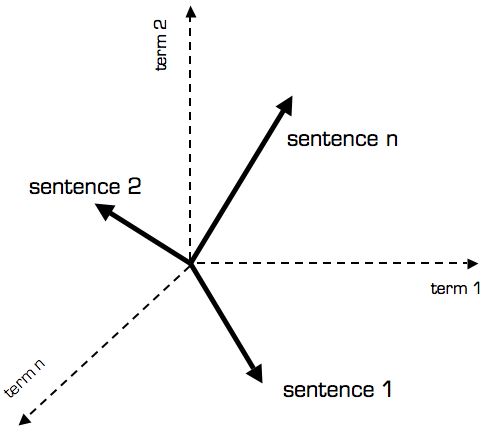
\includegraphics[scale=0.35]{graphics/vector-space.png}
    \end{figure}}
\end{frame}

\begin{frame}{Classification}
    \only<1->{For simplicity, we can reason using a 2D Space.\\ Data can be separated using a \textit{decision boundary}, which is an \textit{hyperplane}. }

    \only<1>{
        \begin{figure}[b]
            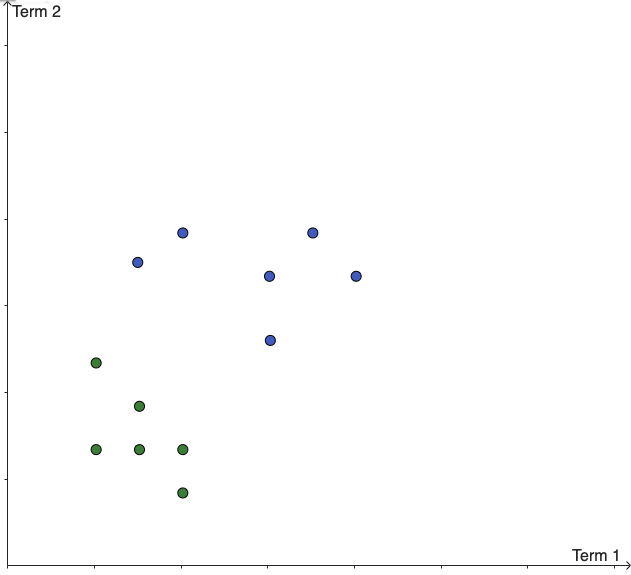
\includegraphics[scale=0.20]{graphics/before.png}
        \end{figure}}
        
    \hspace{-0.17em}
    
    \only<2>{
        \begin{figure}[b]
            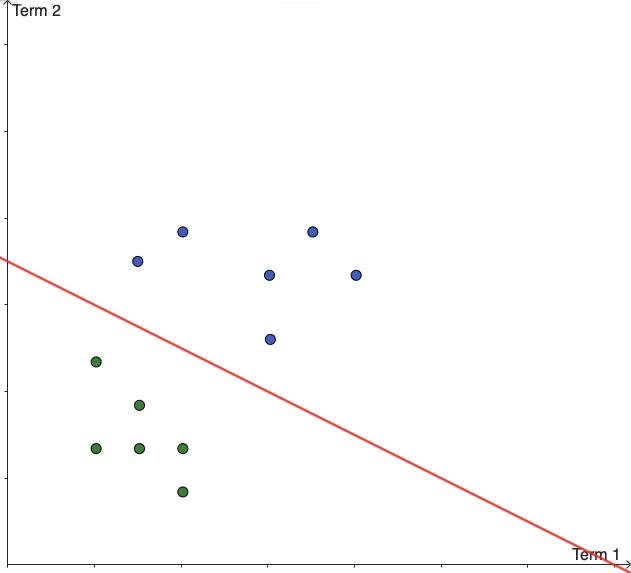
\includegraphics[scale=0.20]{graphics/after.png}
        \end{figure}}

    \hspace{-0.17em}
    
\end{frame}


\begin{frame}{Support Vectors}
    \only<1->{In the previous example the \textit{decision boundary} is a line, represented by the equation~$a + b{t}_{1} + c{t}_{2} = 0$.\\  
    We can introduce two parallels hyperplanes (lines) to the decision boundary, called \textit{support vectors} whose equations are} 
    \only<1->{
    \begin{equation}
        \begin{cases}
          a + b{t}_{1} + c{t}_{2} = 1\\
          a + b{t}_{1} + c{t}_{2} = -1\\
        \end{cases}\
    \end{equation}}

    \uncover<2->{
        \begin{figure}[]
            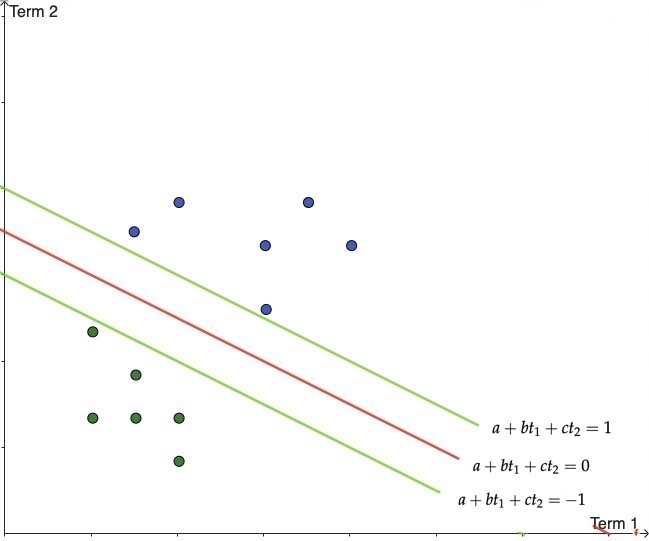
\includegraphics[scale=0.20]{graphics/support vectors.jpg}
        \end{figure}}
    \hspace{-0.1em}
    
\end{frame}

\begin{frame}{Margin}
    \only<1->{For convenience, we can rewrite equations using \textit{vectorization} notation.  
    \begin{equation}
        \begin{cases}
          {b}^Tt + a = 0\\
          {b}^Tt + a = \pm1\\
        \end{cases}\
    \end{equation}}
    
    \uncover<2->{Intuitively, we can define the \textit{margin} of the two support vectors as the distance between them. 
    \vspace{5mm}} %5mm vertical space
    \uncover<3->{\\We can consider two points $x_1,x_2$ that lie respectively on the two support vectors, their distance is~$\lambda\lVert b \rVert = \frac{2}{\sqrt{{b}^Tb}}$. 
    \vspace{5mm} %5mm vertical space
    \\SVM are used to find the \textit{maximum margin linear classifier}, thus we want to maximize the margin.}
     
\end{frame}

\begin{frame}{Cost Function}
    \only<1->{Remembering we want to classify documents, our goal is to find specific $b$ s.t.
    given a document $x$ belonging to class $y$ the decision boundary behave the following:
    \begin{equation}
        \begin{cases}
          {b}^Tx + a \geq 1\qquad if\ y = 1\\
          {b}^Tx + a \leq -1\qquad if\ y = -1\\
        \end{cases}\
    \end{equation}}
    \uncover<2->{We can define the \textit{cost function} as a system of equations.
    \begin{equation}
        \begin{cases}
          \min_{b,a} \frac{\sqrt{{b}^Tb}}{2}\\
          subject\ to \quad y_i(b^Tx_i + a)\geq1 \quad \forall x_i\\
        \end{cases}\
    \end{equation}}
     
\end{frame}

\begin{frame}{Soft-Margin}
    \only<1-3>{In real world problem it is not likely to get an exactly separate line dividing the data within the space. It would be better for the smooth boundary to ignore few data points than be curved or go in loops, around the outliers.}
    \vspace{5mm}
    \uncover<2-3>{\\So, we will use \textit{slack variables} to introduce a penalty for each misclassified point.}
    \vspace{5mm}
    \uncover<3>{\\The new cost function will be
        \begin{equation}
            \begin{cases}
              \min_{b,a} \frac{\sqrt{{b}^Tb}}{2} + C  \sum_{i} \xi_i\\
              subject\ to \quad y_i(b^Tx_i + a)\geq1-\xi_i\quad and\ \xi_i>0 \quad \forall x_i\\
            \end{cases}\
        \end{equation}}
\end{frame}

\begin{frame}{Visualization}
    \only<1->{The larger is C the stricter the classification is, since a larger C will give more evidence to slack variables.
        \begin{equation}
                \begin{cases}
                  \min_{b,a} \frac{\sqrt{{b}^Tb}}{2} + C  \sum_{i} \xi_i\\
                  subject\ to \quad y_i(b^Tx_i + a)\geq1-\xi_i\quad and\ \xi_i>0 \quad \forall x_i\\
                \end{cases}\
            \end{equation}
    }
    \uncover<2->{
        \begin{figure}[b]
            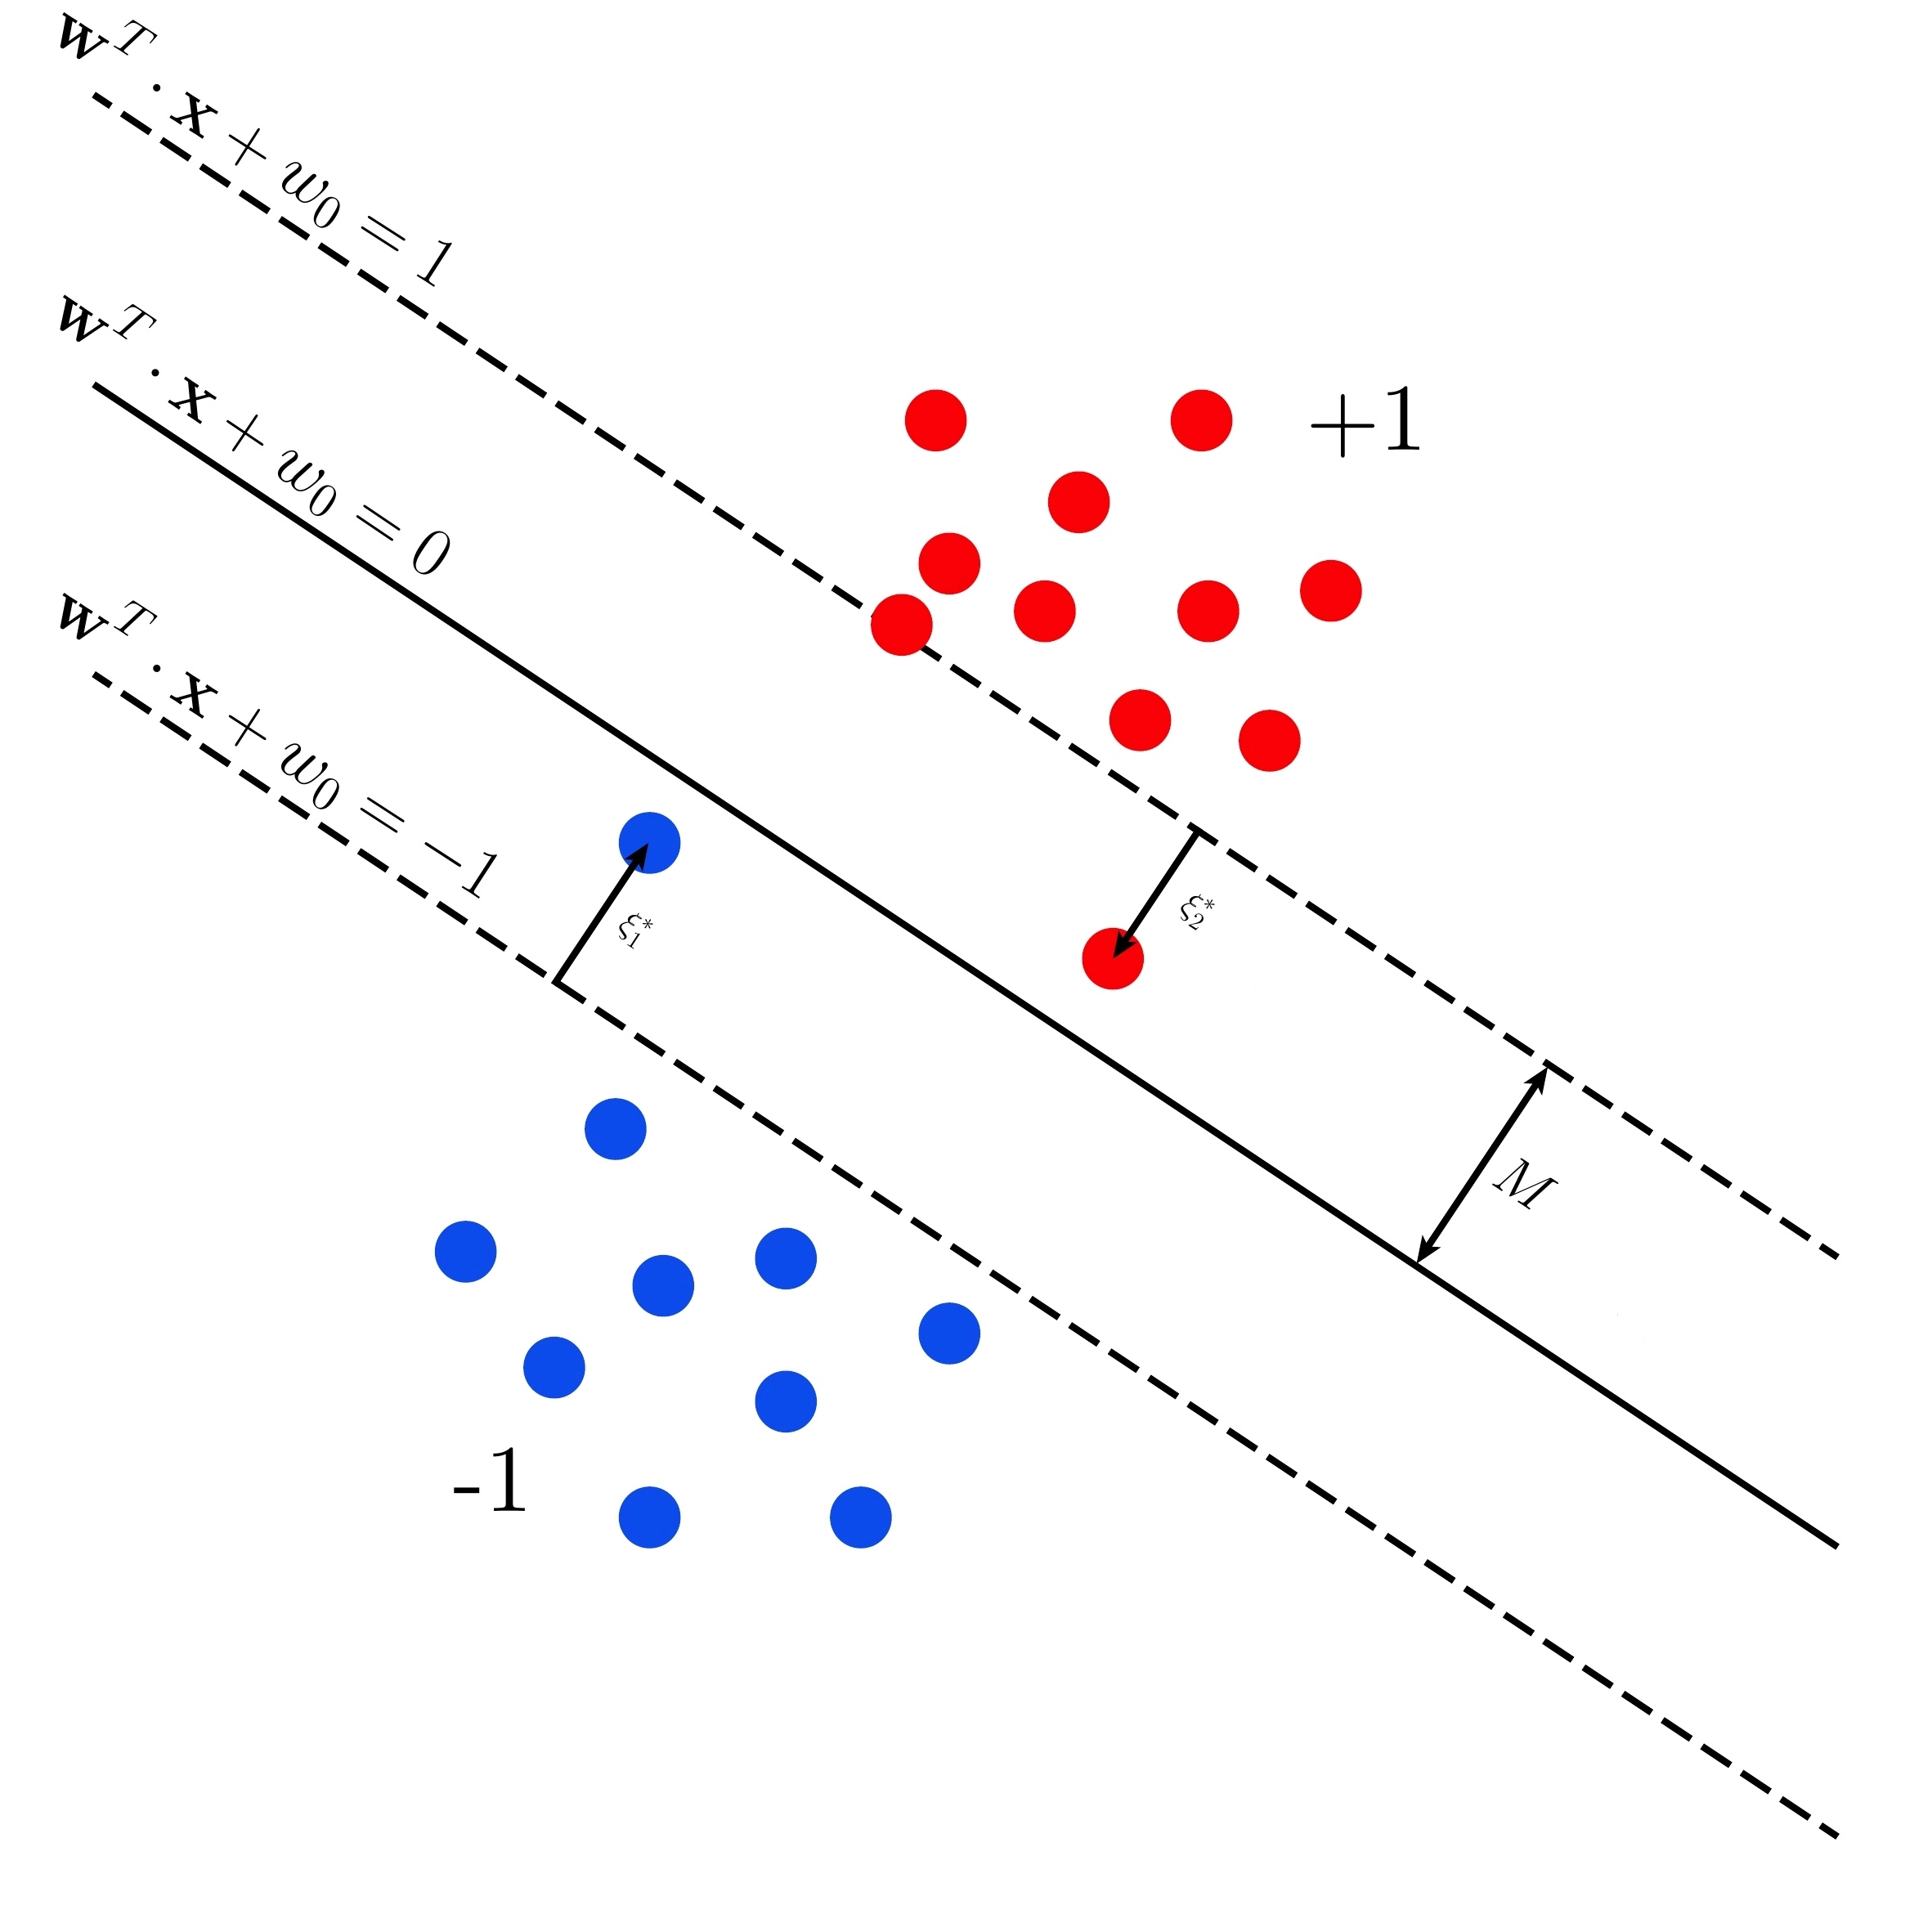
\includegraphics[scale=0.055]{graphics/slack.jpg}
        \end{figure}
    }
\end{frame}

\section{Non linearly separable data}

\begin{frame}{Non linearly separable data}
    \only<1->{What if our data is not linearly separable?}
    \uncover<2->{
     It should be better to reason in a bigger dimensional space.
     \begin{figure}[]
            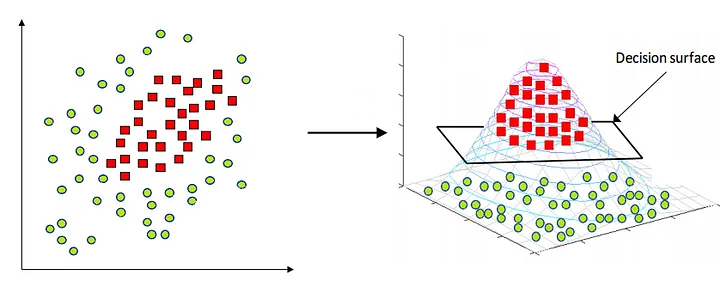
\includegraphics[scale=0.4]{graphics/kernel.jpg}
        \end{figure}
    }
    \uncover<3>{
    But augmenting dimensions costs a lot\ldots
    }
\end{frame}

\begin{frame}{Kernel Trick}
    
    \only<1->{Here \textit{Kernel Trick} comes handy.} 
    \vspace{5mm}
    \uncover<2->{\\Consider the function $\phi : \mathbb{R^3} \mapsto \mathbb{R^{10}}$}
    \vspace{5mm}
    \uncover<3>{\\It allows us to operate in the original feature space without computing the coordinates of the data in a higher dimensional space.}
    
\end{frame}




\end{document}